\subsection{Full Rate DFE}
\subsubsection*{Direct implementation}
\begin{itemize}
    \item Low complexity (one summing node).
    \item Difficult in design for flip-flop, DFE Block in high frequency at low power consumption levels.
    \item Condition of critical timing path.
\end{itemize}

\begin{equation}
    t_{cq,FF} + t_{FB} + t_{setup,FF} < UI
\end{equation}

\begin{figure}[h]
    \centering
    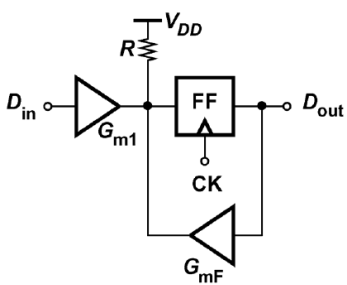
\includegraphics[width=0.5\textwidth]{img/DFE_img/DFE_img_14.png}
    \caption{Full Rate DFE}
\end{figure}

\subsection{Unrolled Full Rate DFE}
\begin{itemize}
    \item High complexity (two summing node, Mux).
    \item Relaxes critical timing path.
    \item Condition of critical timing path.
\end{itemize}

\begin{equation}
    t_{cq,FF} + t_{mux} + t_{setup,FF} < UI 
\end{equation}

Although it relaxes the timing constrain of first loop

\begin{figure}[h]
    \centering
    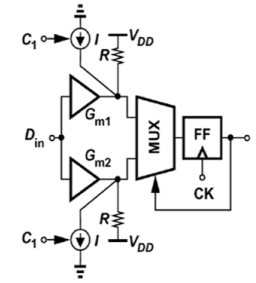
\includegraphics[width=0.4\textwidth]{img/DFE_img/DFE_img_15.png}
    \caption{Unrolled Full Rate DFE}
\end{figure}

\subsection{Half Rate DFE}
\begin{itemize}
    \item High complexity (two summing node).
    \item Larger area and power.
    \item Condition of critical timing path.
\end{itemize}

\begin{equation}
    t_{cq,FF} + t_{FB} + t_{setup,FF} < UI 
\end{equation}

The timing here is the same as the timing Full rate DFE. The principal advantage of this architecture is the simpler design of the CDR circuit, the clock buffer and the flip flops.

\begin{figure}[h]
    \centering
    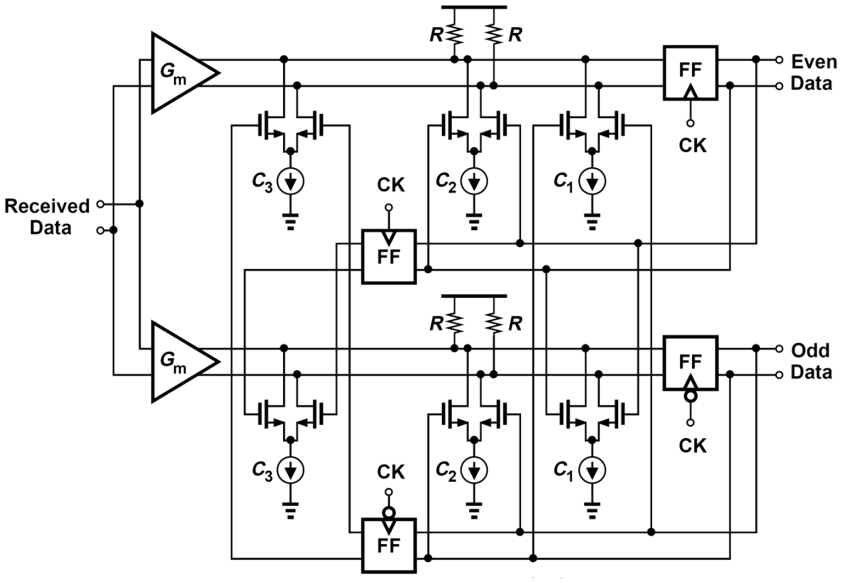
\includegraphics[width=0.6\textwidth]{img/DFE_img/DFE_img_16.png}
    \caption{Half-Rate DFE}
\end{figure}

\subsection{Half Rate Loop-Unrolled DFE}
\begin{itemize}
    \item Relaxes timing constraints
    \item Reduces loading at summing nodes comparable with Direct Half Rate (as for the first tap is only current source subtracting or adding)
    \item High complexity
    \item Four summing nodes
    \item Condition of critical timing path.
\end{itemize}

\begin{figure}[h]
    \centering
    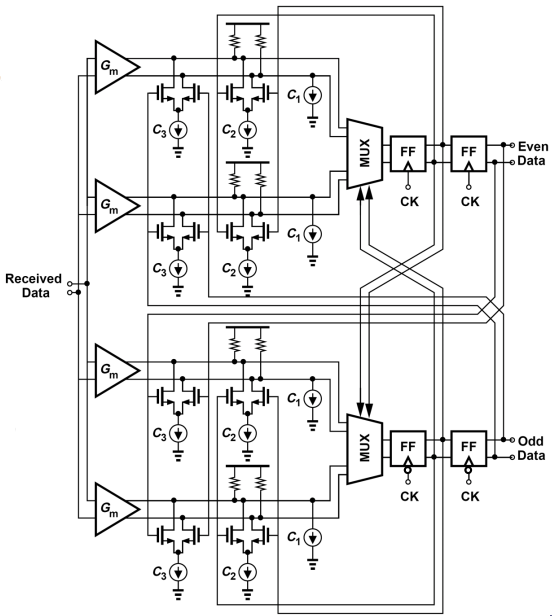
\includegraphics[width=0.5\textwidth]{img/DFE_img/DFE_img_17.png}
    \caption{Half Rate Loop-Unrolled DFE \cite{park2007}}
\end{figure}

\begin{equation}
    t_{cq,FF} + t_{mux} + t_{setup,FF} < UI 
\end{equation}


\subsection{Multiplexed Half Rate DFE}
\begin{itemize}
    \item Half-rate clock
    \item Larger delay
    \item Saves one summing node
    \item Condition of critical timing path.
\end{itemize}

\begin{equation}
    t_{cq,FF} + t_{FB} + t_{mux} + t_{setup,FF} < UI 
\end{equation}

\begin{figure}[h]
    \centering
    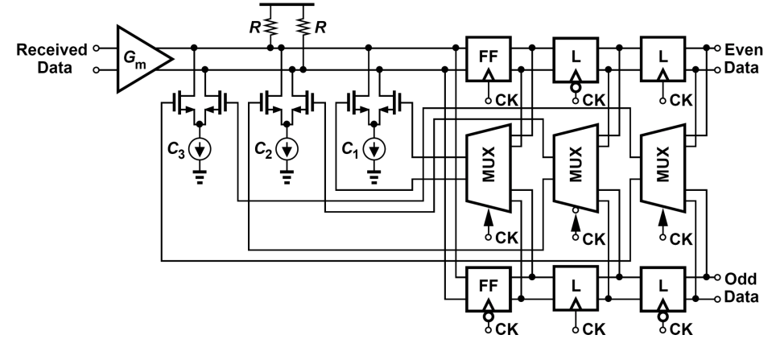
\includegraphics[width=0.7\textwidth]{img/DFE_img/DFE_img_18.png}
    \caption{Multiplexed Half Rate DFE \cite{payne2005}}
\end{figure}

\subsection{Half Rate Loop-Unrolled Multiplexed DFE}
\begin{itemize}
    \item Multiplexer to choose between odd and even (saving 2 summing nodes)
    \item Multiplexer to choose whether bit is 0 or 1
    \item Saving two summing nodes
    \item Condition of critical timing path.
\end{itemize}

\begin{figure}[h]
    \centering
    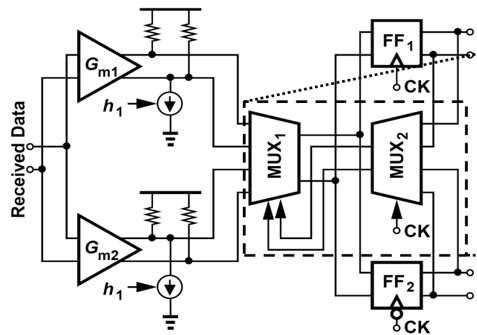
\includegraphics[width=0.5\textwidth]{img/DFE_img/DFE_img_19.png}
    \caption{Half Rate Loop-Unrolled Multiplexed DFE \cite{ibrahim2010}}
\end{figure}

\begin{equation}
    t_{cq,FF} + t_{FB} + t_{mux1} + t_{mux2} + t_{setup,FF} < UI 
\end{equation}


\subsection{Quarter-Rate DFE}
For extremely high speeds, a Quarter-Rate architecture uses four parallel paths driven by quadrature clocks (0, 90, 180, 270 degrees). But at the cost of much larger area and power.

\begin{figure}[h]
    \centering
    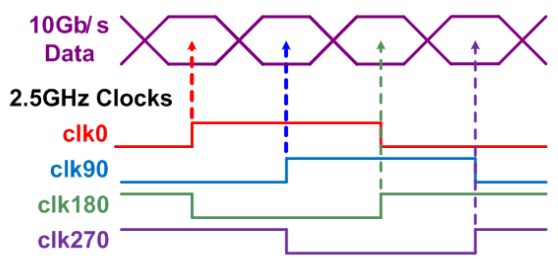
\includegraphics[width=0.4\textwidth]{img/DFE_img/DFE_img_20.png}
    \caption{(a) Quarter-Rate DFE}
\end{figure}

\begin{figure}[h]
    \centering
    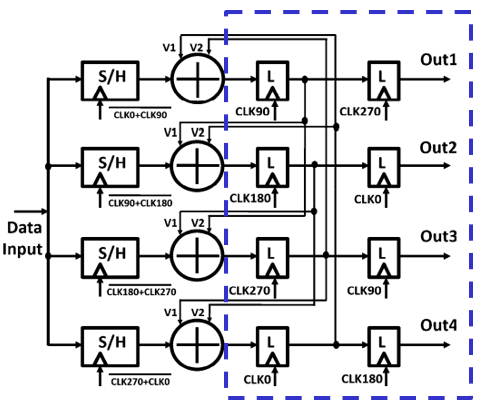
\includegraphics[width=0.4\textwidth]{img/DFE_img/DFE_img_21.png}
    \caption{Quarter phase CLK}
\end{figure}

\subsection{DFE IIR Equalization}
As mentioned in [3]. If we have a smooth channel, we can make IIR filter instead of FIR and saving many taps and better performance.

\begin{figure}[H]
    \centering
    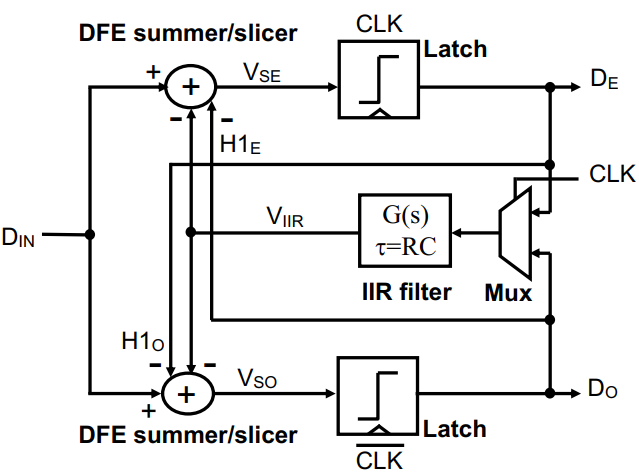
\includegraphics[width=0.45\textwidth]{img/DFE_img/DFE_img_12.png}
    \hfill
    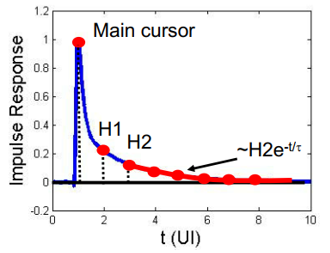
\includegraphics[width=0.45\textwidth]{img/DFE_img/DFE_img_13.png}
    \caption{(a) 1-tap DFE with IIR Filter (b) Impulse response}
\end{figure}

\subsection{DFE Summing Node Design}
The summer circuit is responsible for subtracting the ISI currents from the input signal. Its performance is characterized by its settling time accuracy (>95\%) and bandwidth.

\subsubsection{Resistive-Load Summer}
The conventional summer uses a differential pair with resistive loads. The settling behavior is exponential. A trade-off exists: to decrease the time constant ($\tau = RC$), R must be reduced. However, to maintain the voltage swing ($V = IR$), the bias current I must increase proportionally. This results in high power consumption for high-speed designs.

\begin{figure}[h]
    \centering
    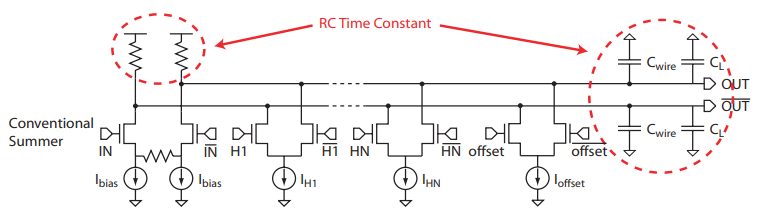
\includegraphics[width=0.8\textwidth]{img/DFE_img/DFE_img_22.png}
    \caption{Resistive-Load Summer \cite{park2007}}
\end{figure}

\subsubsection{Integrating Summer}
To overcome the RC bandwidth limitation, \textbf{Integrating Summers} are used. These circuits replace the load resistors with capacitors (often parasitic capacitance) and use a reset switch.

Diff output voltage:

\begin{equation}
    \Delta V = I \times \frac{\Delta T}{C}
\end{equation}

\begin{figure}[h]
    \centering
    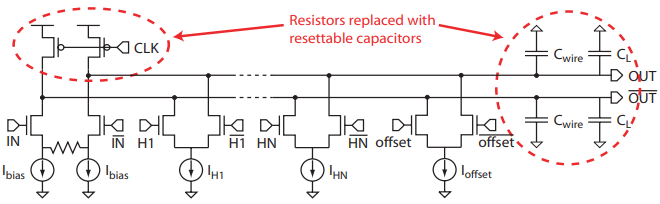
\includegraphics[width=0.6\textwidth]{img/DFE_img/DFE_img_23.png}
    \caption{Integrating Summer \cite{park2007}}
\end{figure}

Since $\frac{\Delta T}{C} > R$, bias current can be reduced for a given output swing. These integrators consume over an order of magnitude less power than the resistively loaded summers. Integrating summers provide linear settling, which is faster than exponential settling for the same power budget. However, the output common-mode voltage can't be controlled because of I/C ratio variation with process and also counting on parasitic caps or operating at different data rate, which requires Common-Mode Restoration circuit, to prevent the output common-mode voltage from drifting.

\begin{figure}[h]
    \centering
    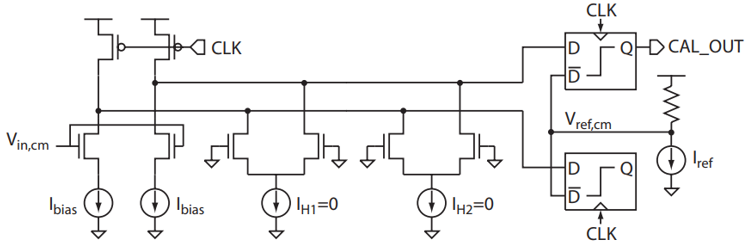
\includegraphics[width=0.6\textwidth]{img/DFE_img/DFE_img_24.png}
    \caption{Common-mode restoration circuit \cite{park2007}}
\end{figure}

\subsection{PAM4 DFE}
PAM-4 DFE requires 3 slicers to compare as the symbol contains 2 bits (4 levels). Requires thermometer to binary also to minimize number of latches. Each tap has four possible values ($\pm h , \pm 3h$)

\textbf{In 1-tap Unrolling PAM-4 DFE:}
\begin{itemize}
    \item DFE requires 12 data slicers because the previous symbol has four possible outcomes (4× for each DH, DZ, and DL) and 3 MUXs.
    \item Requires thermometer to binary to select the required input from MUX
\end{itemize}

\begin{figure}[h]
    \centering
    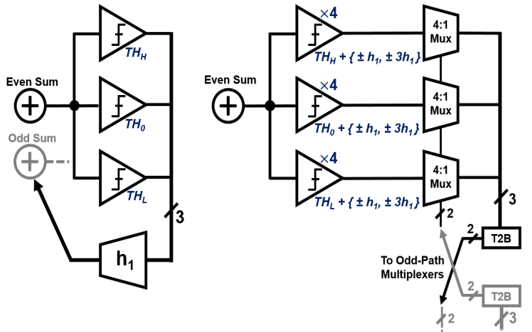
\includegraphics[width=0.5\textwidth]{img/DFE_img/DFE_img_25.png}
    \caption{(left) Half Rate PAM4 DFE (right) Half Rate Loop-Unrolled PAM4 DFE chen2020}
\end{figure}